%
% tp 2 mna
% 

% Use emulateapj instead to make Apj format.
% YOU SHOULD REMOVE THE TABLE OF
% CONTENTS PAGE WHEN USING APJ FORMAT.
\documentclass[11pt,a4paper]{emulateapj}
\bibliographystyle{apj}


%define general packages
\usepackage{epsfig}
\usepackage{amsmath}
\usepackage{natbib}
\usepackage{graphicx}


% spanish packages
\usepackage[utf8]{inputenc}
\usepackage[spanish]{babel}
\languageshorthands{none}
\noextrasspanish
\let\layoutspanish\relax
\usepackage[spanish]{babel}
\renewcommand\shorthandsspanish{}

%internal short cuts
\def \HgA {H$\gamma_A$}
\def \gon {Gonz\'{a}lez}
\def \Hbp {H$\beta ^\prime$}
\def \warn {{\sffamily\bfseries\large WARNING, ARREGLAR:}}









\begin{document}

\submitted{Departamento Ing. en Informática, ITBA}
\title{Filtros espaciales en imagenes mediante el paso del dominio espacial al dominio de las frecuencias}
\author{Williams M. \& Aráoz M.}
\date{\today}


\begin{abstract}
\warn{hacer abstract}
\end{abstract}

\maketitle




\section{Introduccción}
\label{sec:introduccion}

%\begin{figure*}
%  \begin{center}
%    \leavevmode
%      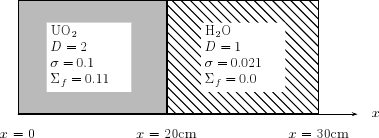
\psfig{file=images/img1.png, width=254px}
%       \caption[Esquema simple del reactor]{Modelo de un ractor nuclear unidimensional.
%         Diagrama adaptado de \citet{diaz10}.}
%     \label{fig:esquema}
%  \end{center}
%\end{figure*}





Dada una señal cualquiera, una representación en el dominio del tiempo muestra como evoluciona dicha señal
a través del tiempo. Por otro lado, una representación en el dominio de las frecuencias muestra qué tanto de 
la señal pertenece a cada banda de frecuencias en un determinado rango. \citet*{wiki10} Una función o señal puede ser convertida
o "transformada" entre el dominio del tiempo y la frecuencia mediante operadores funcionales introducidos por 
Joseph Fourier para el estudio de la difusión del calor. Dichos operadores son la transformada de Fourier (para
pasar una función del dominio del tiempo al dominio de la frecuencia) y la antitransformada de Fourier (para hacer
el proceso inverso). Ambos operadores descomponen una función en una suma infinita de senos y cosenos, o equivalentemente
en una suma de funciones exponenciales complejas. \\

Las ecuaciones que permiten estos operadores son: \\
\begin{eqnarray}
\mathcal{F}\{f\} &=& \dfrac{1}{2\pi} \int_{-\infty}^{\infty} f(x)e^{-2\pi i \omega x} dx  \\
\check{f} &=& \dfrac{1}{2\pi} \int_{-\infty}^{\infty} f(x)e^{2\pi i \omega x} dx
\end{eqnarray}
donde $\mathcal{F}\{f\} $ representa la transformada de Fourier de $f$ y $\check{f}$ la antitransformada de Fourier de $f$.
\citet*{wolf10}\\


La transformada de Fourier puede ser extendida a 2 dimensiones para permitir la transformación de una imagen 
del dominio de los pixels (espacial) al dominio de las frecuencias. Esto permite la aplicación de algunos filtros
espaciales con algunas ventajas en performance debido a que es más eficiente computar la transformada
de Fourier, realizar productos en el dominio de las frecuencias, y computar la transformada inversa,
que computar la convolución en el dominio espacial.\citet*{bou98} \\

Una imagen (cuadrada, para simplificar el análisis, aunque puede extenderse fácilmente a imágenes rectangulares)
puede definirse matemáticamente como:
\begin{eqnarray}
f:D \times D \rightarrow P
\end{eqnarray}
donde $D \subseteq  \mathbb{N} $ y representa el dominio de un lado de la imagen (alto o ancho), 
y $P$ representa el espacio de pixels (valores típicos son $P=[0,255]\cap\mathbb{N}$ para imágenes
en escala de grises o $P=[0,16581375]\cap\mathbb{N}$ para imágenes a color). \\

De esta forma, la imagen es representada por la función $f$ haciendo que $f(x,y)$ represente el color
del pixel en la posición $(x,y)$ de la imagen. \\

Por esta forma de representar la imagen, es necesario discretizar los operadores de transformada y 
antitransformada de Fourier en 2 dimensiones. Esto se logra mediante las siguientes ecuaciones, suponiendo que el conjunto $P$ del codominio de la imagen $f$ tiene un cardinal igual a $card(P)= N$.

\begin{eqnarray}
T_{l,k} &=& \sum_{n=0}^{N-1}\sum_{m=0}^{N-1} I_{n,m}e^{-\frac{2\pi i}{N}(nl+mk)} \\
I_{n,m} &=& \dfrac{1}{N^2}\sum_{l=0}^{N-1}\sum_{k=0}^{N-1} X_{l,k}e^{\frac{2\pi i}{N}(nl+mk)} 
\end{eqnarray}
donde $T_{l,k} $ representa la transformada de Fourier de la imagen $I$ y $I_{n,m} $ la antitransformada de Fourier de la imagen.\\

Así, se pueden aplicar filtros espaciales usando estas ecuaciones discretizadas. Para esto, se transforma la imagen
al dominio de las frecuencias, se aplica el filtro (mediante una multiplicación) y luego se antitransforma la imagen
al dominio espacial para ver el resultado.

\section{Filtros utilizados}
\label{sec:sec2}
Para este trabajo utilizamos 3 filtros. El primero lo llamamos Pulso y cumple la esta definido por la siguiente función:

\begin{eqnarray}
H(k,l) = \left\{
	\begin{matrix}
		0, 0 \leq k \leq 400, 190 \leq l \leq 210 \\
		0, 0 \leq l \leq 400, 190 \leq k \leq 210 \\
		1, \quad $resto de las posiciones$
	\end{matrix} 
	\right.
\end{eqnarray}
Este filtro tiene la forma de una cruz y filtra las frecuencias altas en ambas variables. No filtra las frecuencias altas en
una sóla variable (en las cuales la otra variable tiene baja frecuencia). Esto produce un efecto similar al filtro
pasaaltos.\\
El segundo filtro que utilizamos es el llamado Gaussiano:

\begin{eqnarray}
H(k,l) = e^{-0.1(k^2 + l^2)}
\end{eqnarray}
El filtro gaussiano lo que hace es aplicarle una difusión a la imagen. Es decir cambiando el valor por cual está multiplicado, la suma de los cuadrados de las variables, se puede variar la profundidad de la difusión. Es decir, al hacer ese valor más chico en valor absoluto, se logra una imagen menos difusa, pero al agrandar ese valor, la imagen obtenida se vuelve cada vez más difusa. Esto se debe a que el filtro gaussiano funciona como un filtro pasabajos, anulando las altas frecuencias, que es lo que da la sensación de bordes en las imágenes.
\\
El último filtro utilizado es el que llamamos Damero:
\begin{eqnarray}
H(k,l) = \left\{
	\begin{matrix}
		0,$ si $l+k$ es par$\\
		1,$ si $l+k$ es impar$\\
	\end{matrix} 
	\right.
\end{eqnarray}
El filtro damero o checkerboard filtra los pixels alternados, como en un tablero de ajedrez. Esto produce que se 
filtren (se apaguen) algunas frecuencias salteadas, causando un comportamiento altamente no lineal en el dominio
del espacio.


\section{Codigo utilizado}
\label{sec:sec3}
Para llevar a cabo este trabajo utilizamos un \emph{script} para aplicar los filtros. A su vez, los filtros también se encuentran escritos como funciones de \emph{Matlab/Octave}. El código que aplica los filtros se puede ver en la figura Fig. \ref{fig:codigobase}, y podemos hacer unos comentarios al respecto. 
\begin{figure}
      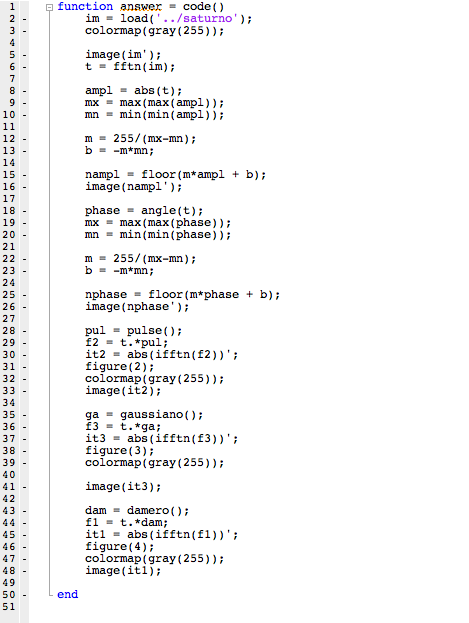
\includegraphics[width=254px]{images/code.png}
       \caption[Código utilizado para aplicar los filtros.]{Código utilizado para aplicar los filtros.}
     \label{fig:codigobase}
\end{figure}
En primer lugar, para calcular la Transformada de Fourier en varias dimensiones, hacemos uso de la función \emph{fftn} de \emph{Matlab}, que según la documentación utiliza el algoritmo FFTW para computar la Transformada Discreta de Fourier. Asimismo, la antitransformada se calcula utilizando la función \emph{ifftn}, que también la provee \emph{Matlab}. Es necesario remarcar que para se vea una imagen al dibujar los puntos que se encuentran en el archivo \emph{Saturno}, se tiene que setear el mapa de colores en una escala de grises desde 0 al 255. Esto es porque cada punto del archivo representa un número de gris entre 0 y 255. Por la misma razón, luego de que calculamos la fase y la amplitud, normalizamos los valores obtenidos entre 0 y 255.

\section{Resultados y Conclusiones}
\label{sec:resultadosyconclusiones}
Como resultados de este trabajo, obtuvimos las imagenes luego de aplicar los filtros. Todas las imagenes se obtuvieron luego de aplicar filtros a la imagen original que se muestra en Fig. \ref{fig:imagensaturno}. 
\begin{figure}[ht!]
     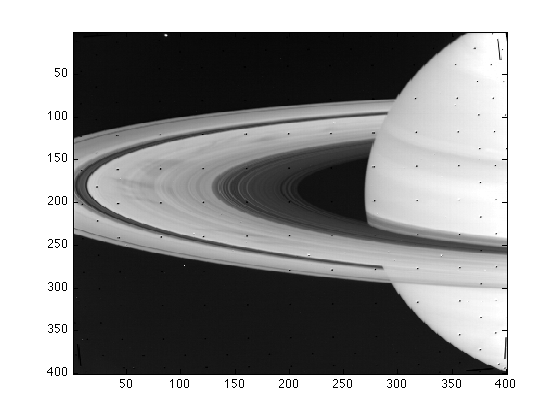
\includegraphics[width=254px]{images/saturno.png}
      \caption[Imagen original de Saturno.]{Imagen original.}
     \label{fig:imagensaturno}
\end{figure} 
Primero veamos la imagen obtenido luego de aplicar el filtro Gaussiano. En la figura Fig. \ref{fig:imagengaussiana} se puede la imagen original pero difusa. Es decir, no se distingue con claridad la imagen de Saturno.
\begin{figure}[ht!]
     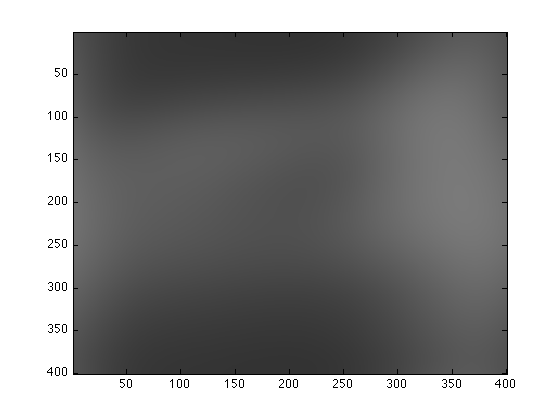
\includegraphics[width=254px]{images/gaussiano.png}
       \caption{Imagen resultante de la aplicación un filtro Gaussiano.}
     \label{fig:imagengaussiana}
\end{figure} 
En segundo lugar, veamos la imagen obtenida luego de aplicarle un filtro damero, que se muestra en la Fig. \ref{fig:imagendamero}. En este caso se puede ver el comportamiento no lineal que produce el filtro a la imagen.
\begin{figure}[ht!]
     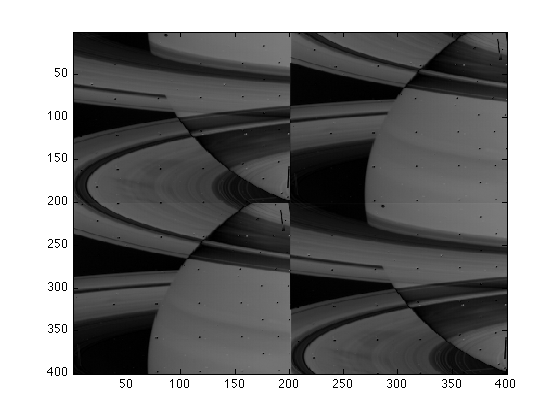
\includegraphics[width=254px]{images/damero.png}
       \caption{Imagen resultante de la aplicación un filtro Damero.}
     \label{fig:imagendamero}
\end{figure} 
Por último veamos el resultado de aplicar un filtro Pulso a la imagen original. En la figura Fig. \ref{fig:imagenpulse} se puede ver el resultado. Es interesante ver que además de generar un efecto sobre el contenido de la imagen, también cambia los colores de la misma.
\begin{figure}[ht!]
     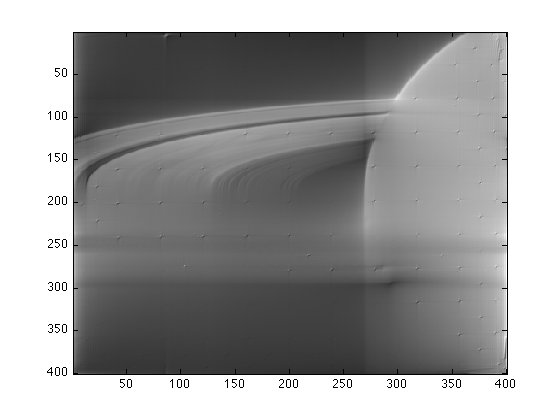
\includegraphics[width=254px]{images/pulse.png}
       \caption{Imagen resultante de la aplicación un filtro Pulso.}
     \label{fig:imagenpulse}
\end{figure} 

%
\bibliography{paper}

\end{document}

